\documentclass[twoside]{uva-inf-bachelor-thesis}
%\usepackage[dutch]{babel}

% Filling your thesis with only lorem ipsum is not advised.
\usepackage{lipsum}

% Title Page
\title{Title}
\author{Lennaert Feijtes}
\email{contact@ludof.nl - lennaert.feijtes@student.uva.nl}
\supervisors{Supervisors}
\signedby{Signees}

\begin{document}
\maketitle

\begin{abstract}

This research examines how text redaction in PDF documents can be accomplished while effectively addressing security concerns and preserving non-redacted text. 

Our findings reveal that a method can be created which both ensures confidentiality of sensitive information and the preservation of the non-redacted text. While file .... Using a sample of both custom and real world PDF documents in the Edact-Ray Tool Suite, we have tested our method on adhering to the safety concerns and possible leaking of information. Our findings reveal that no information is being leaked using our method...

The results highlight that a tool for safe text redaction is possible and that information can be kept confidential while maintaining semantic context in the document. 

This study contributes to...
\end{abstract}

\tableofcontents

% https://practicumav.nl/schrijven/schrijfstijl.html

\chapter{Introduction}
ok
\chapter{Related work}

\cite{bland2022story} presents a method for breaking PDF text redaction using glyph positions; non-redacted character positioning information. In particular, subpixel-sized horizontal shifts in both the redacted and non-redacted characters can be recovered and used to effectively deredact first and last name. Breaking text-redaction schemes relies on knowing the position of characters on the page, something that is important to consider when redacting directly in a PDF instead of scanning and then OCR-ing documents. While this paper only focuses on names which may be derived from both the positioning information and potential candidates from publicly available data, this method may also be suitable for attacking other sensitive information with a reasonable length; email-addresses, phone numbers and postal addresses.
\\\\
Redaction through mosaicing and blurring where text is significantly distorted and transformed such that it is unrecognizable for the eye are popular, especially for images shared through social media. Mosaicing (pixelization) and blurring have been proven to not be viable techniques for text redaction (figure \ref{fig:blurredredaction}). Due to particular regularities in text, enough information may remain to narrow down the possibilities or even to recover the redacted text \cite{hill2016effectiveness}. A simple but powerful class of statistical models, Hidden Markov Models, can be used to recover both short and indefinitely long instances of redacted text. HMMs are used to reover sequences of characters from images of redacted text. 
\begin{figure}[h]
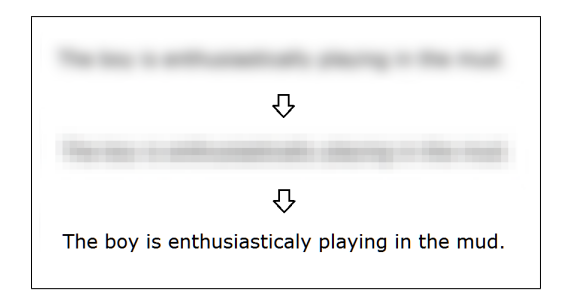
\includegraphics[width=0.7\textwidth]{latex/media/blurredRedaction.png}
\centering
\caption{Example of how a blurred image is first mosaiced, and then the text is inferred by an HMM. Not a viable option for text redaction in documents.}
\label{fig:blurredredaction}
\end{figure}
\\\\
Several methods and tools have been created to automatically find different types of redacted text in PDF documents. The X-Ray Bad Redaction Detector (X-RAY) is a fast and robust tool to identify bad redactions in PDF files \cite{Xray2021}. X-RAY detects trivial redactions where text is badly redacted under a rectangle. A technique using a combination of OCR and morphological operations has been created to detect a wide variety of different types of redaction blocks \cite{van2023detection}.
\\\\
There are several (commercially) available redaction tools which are used for text redaction and anonymization. Octobox \cite{OCTOBOX} and Zylab \cite{Zylab} are two tools frequently used by governmental bodies and municipalities in The Netherlands. \textbf{more about this}

\chapter{Design}

\section{Portable Document Format}
In the context of text redaction, it is essential to consider the relevant components that make up a PDF document and influence security for direct redaction in the document. We consider the PDF document type which contains text data for both the font and the layout of each character (glyph) on a page. 

\subsection{Structure}
A PDF document can be split into 4 distinct parts: 
\\\\
\textbf{Header}. The header of a PDF document serves as its starting point. It contains the critical information about the file which is essential for identifying the PDF format and ensuring compatibility with PDF readers. \\
\textbf{Trailer}. The trailer is found at the end of the document and provides essential information for reading and processing the document. It includes the number of entries in the cross-reference table. It references to the root object of the document's catalog, which contains information about the document's structure, outlines and elements. Finally it may include additional information about encryption, digital signatures and metadta if present. \\
\textbf{Cross-Reference Table(Xref)}. The Cross-Reference Table maintains a record of the location and structure of all objects within the PDF. The Xref table enables efficient random access and editing of the document. It lists the objects, their byte offsets within the file and information about whether an object is in use of has been deleted. \\
\textbf{Body}. The body is where the actual content resides. It includes everything that is visible within the document. This includes text, images, graphical elements, forms and more. The content of a PDF is organized into objects. 
\\\\
The actual contents of a page are often embedded through a stream. A stream may be contained in an object and consists of a sequence of operators with operands which may refer to other objects or information elsewhere.
\begin{figure}[h]
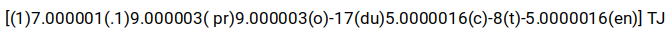
\includegraphics[width=0.85\textwidth]{latex/media/TJexample.png}
\centering
\caption{The TJ text showing operator specifies the glyphs to render, along with their widths and associated positional adjustments by the reference to a font object (not shown here). Adjustments are given in text space units. }
\label{fig:tjexample}
\end{figure}
\subsection{Text rendering}
PDF documents can render text in a wide range of ways, including by the use of a text showing operator such as TJ or Tj. The TJ operator takes as arguments a string of text and a vector of positional adjustments which displace the character with respect to its default position. This position is often determined by the previous character on the line, consisting of a fixed offset that is equivalent to the \textit{advance width} of the previous character. Figure \ref{fig:tjexample} is an example of a TJ text showing operator in practice.
\\\\
Glyph advance widths and glyph shifts create a security concern. The exact width of a redaction and any non-redacted glyph shifts conditioned on redacted glyphs may be used to eliminate potential redacted texts. \cite{bland2022story}. Documents may or may not have these positional adjustments based on the \textit{workflow} that has been used. When saving an email or using 'Save as PDF' in Microsoft Word for example, the documents have \textit{dependent} shifting schemes, while other workflows may produce documents which are \textit{unadjusted}.

\subsubsection{Redaction width}


\subsection{Metadata}
A PDF document may contain extra 'hidden' information which is contained within the metadata of the document. This metadata may contain information about the actual textual contents of the document (figure \ref{fig:metadataexmp}). An example are annotations by authors or reviewers which may comment on a specific part of the document, referring or quoting text which has been redacted from the page, but not from the document. 
\begin{figure}[h]
    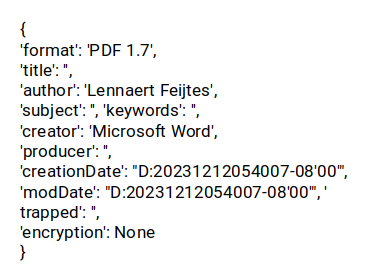
\includegraphics[width=0.5\linewidth]{latex/media/metadata.png}
    \centering
    \caption{An example of metadata which may be present in a PDF document. Information such as the author name, subject and description of the document can be retrieved if not also removed.}
    \label{fig:metadataexmp}
\end{figure}\\
The table of contents, embedded files, XML metadata and internal links are also hidden to the eye but may contain sensitive information even after redaction. This information may include author names, document descriptions, links or other references to sensitive personal information which has not been correctly removed.

\section{Steps of possible redaction}
The process of safely redacting information from a document consists of multiple steps. To redact text, it first has be labeled as text that should be redacted in order to differentiate it from text that should not be removed. It is also important to differentiate between whole words and sub-strings of text elements so that exactly that what should be deleted is really removed from the document. Furthermore, a document can consist of multiple pages, so it should be known what set of possible redactions belongs to which page. 
\\\\
The next step is locating the text that has to be removed. As mentioned, text is rendered by a sequence of commands in a content stream. The position of a text element and even an individual character can be reconstructed with these commands. In order to find the location of a text element the commands in the content streams have to be read, parsed and interpreted. There are various ways of rendering text in PDF documents, some more complex than others, and thus it requires a lot of research and work to handle all possible options. 
\\\\
If text positions have been retrieved from a document, text can be removed. To redact, and thus to remove, text from a document, the commands that enable it to be rendered should be removed. Both the text rendering operation and other operations that may influence style and positioning should be removed completely. However, there is no guarantee that text is rendered in a certain way. Text on one line may consist of multiple text rendering operations or just one. Words may be individually grouped or each individual character is rendered separately. Again, this is dependent on the 'producer' of the file and the 'workflow' used. 
\\\\
\textbf{two images with examples of different text rendering styles based on found in the wild}
\\\\
If text has been removed, possible positional information of the other words on the line have to be adjusted to reduce the leaked information. \textbf{add more...} Again, because of the diversity of ways text can be rendered, it may get complex. 
\\\\
For small words


% references
\bibliographystyle{ACM-Reference-Format}
\bibliography{bibliographies/references}
\end{document}
